%%%%%%%%%%%%%%%%%%%%%%%%%%%%%%%%%%%%%%%%%%%%%%%%%%%%%%%%%%%%%%%%%%%%%%%%%%%%%%%%
%% LBS/DR Indoor Positioning System - Academic Paper
%% Multi-Sensor Fusion for Indoor Positioning Using EKF and Particle Filtering
%%%%%%%%%%%%%%%%%%%%%%%%%%%%%%%%%%%%%%%%%%%%%%%%%%%%%%%%%%%%%%%%%%%%%%%%%%%%%%%%

\documentclass[journal,twocolumn]{IEEEtran}

\usepackage[utf8]{inputenc}
\usepackage[T1]{fontenc}
\usepackage{amsmath,amssymb,amsfonts}
\usepackage{algorithmic}
\usepackage{algorithm}
\usepackage{graphicx}
\usepackage{textcomp}
\usepackage{booktabs}
\usepackage{multirow}
\usepackage{cite}
\usepackage{hyperref}
\usepackage{tikz}
\usetikzlibrary{shapes,arrows,positioning,fit,calc}

\begin{document}

\title{Multi-Sensor Fusion Architecture for Indoor Positioning: Integrating Extended Kalman Filtering, Particle Filtering, and Pedestrian Dead Reckoning on Modern Mobile Platforms}

\author{
\IEEEauthorblockN{Semih Dalgin}
\IEEEauthorblockA{Department of Geomatics Engineering\\
Istanbul, Turkey}
}

\maketitle

%===============================================================================
% ABSTRACT
%===============================================================================
\begin{abstract}
Indoor positioning remains a fundamental challenge in location-based services due to the unavailability of Global Navigation Satellite System (GNSS) signals within enclosed structures. This paper presents a comprehensive multi-sensor fusion architecture for indoor positioning that integrates Pedestrian Dead Reckoning (PDR), barometric floor detection, Wi-Fi Round-Trip Time (RTT) ranging, and Bluetooth Low Energy (BLE) beacon proximity into a unified positioning engine. The proposed system employs a dual-filter fusion strategy combining an Extended Kalman Filter (EKF) for state estimation with a Particle Filter (PF) for radio-frequency-based positioning, yielding robust performance across diverse indoor environments. An adaptive step detection algorithm based on the Weinberg stride length model replaces traditional peak-counting methods, while a hypsometric formula-based floor detector supersedes linear pressure-altitude approximations. The architecture is implemented on the Android platform using modern reactive programming paradigms (Kotlin Coroutines and Flow) within a clean layered architecture. Comparative analysis against a legacy Java-based implementation demonstrates improvements in modularity, extensibility, and algorithmic accuracy. The system achieves floor detection confidence exceeding 90\% under stable atmospheric conditions and supports sub-meter horizontal positioning when Wi-Fi RTT infrastructure is available.
\end{abstract}

\begin{IEEEkeywords}
Indoor positioning, sensor fusion, Extended Kalman Filter, Particle Filter, pedestrian dead reckoning, Wi-Fi RTT, BLE beacons, barometric altimetry, floor detection, mobile computing
\end{IEEEkeywords}

%===============================================================================
% I. INTRODUCTION
%===============================================================================
\section{Introduction}

\IEEEPARstart{T}{he} proliferation of location-based services (LBS) has generated significant demand for accurate positioning in environments where Global Navigation Satellite Systems (GNSS) are unavailable or severely degraded. Indoor environments---including shopping malls, airports, hospitals, and multi-story buildings---present particularly challenging scenarios due to signal attenuation, multipath propagation, and the absence of direct satellite line-of-sight \cite{zafari2019survey}.

Traditional outdoor positioning relies on GNSS receivers that achieve meter-level accuracy under open-sky conditions. However, GNSS signal strength attenuates by 20--30~dB upon penetrating building materials \cite{groves2013principles}, rendering satellite-based positioning impractical for indoor applications. This limitation has motivated extensive research into alternative positioning technologies, including Wi-Fi fingerprinting, Bluetooth Low Energy (BLE) beacons, Ultra-Wideband (UWB) ranging, inertial measurement units (IMU), and barometric pressure sensors \cite{davidson2017survey}.

No single sensor technology provides sufficient accuracy and reliability for universal indoor positioning. Wi-Fi and BLE signal strength (RSSI) measurements suffer from environmental variability, with standard deviations of 5--10~dBm observed in typical indoor settings \cite{he2016wifi}. Inertial sensors provide high-rate motion estimation but accumulate drift over time. Barometric sensors enable vertical positioning but are affected by atmospheric pressure variations. This inherent limitation of individual technologies has driven the development of multi-sensor fusion approaches that combine complementary information sources to achieve robust positioning \cite{harle2013survey}.

This paper presents the design, implementation, and analysis of a modern multi-sensor fusion architecture for indoor positioning. The system integrates:
\begin{itemize}
    \item \textbf{Pedestrian Dead Reckoning (PDR)} using accelerometer-based step detection with adaptive stride length estimation;
    \item \textbf{Barometric floor detection} using the hypsometric formula with moving-average smoothing;
    \item \textbf{Wi-Fi RTT (802.11mc)} ranging for sub-meter distance estimation to compatible access points;
    \item \textbf{BLE beacon} RSSI-based proximity estimation;
    \item \textbf{Extended Kalman Filter (EKF)} for optimal state estimation;
    \item \textbf{Particle Filter (PF)} for handling the non-linear, non-Gaussian nature of RF-based positioning.
\end{itemize}

The proposed architecture represents a complete redesign of an earlier indoor positioning system \cite{dalgin_legacy} that was built on legacy Android technologies (Java, API level 15, Maven build system). The new system leverages modern mobile development paradigms---Kotlin coroutines for asynchronous sensor data streams, Jetpack Compose for declarative UI, Hilt for dependency injection, and Room for structured data persistence---while substantially improving the underlying positioning algorithms.

The remainder of this paper is organized as follows. Section~\ref{sec:related} reviews related work in indoor positioning and sensor fusion. Section~\ref{sec:architecture} describes the system architecture. Section~\ref{sec:algorithms} presents the mathematical formulations of the positioning algorithms. Section~\ref{sec:implementation} details the implementation on the Android platform. Section~\ref{sec:comparison} provides a comparative analysis with the legacy system. Section~\ref{sec:conclusion} concludes the paper.

%===============================================================================
% II. RELATED WORK
%===============================================================================
\section{Related Work}
\label{sec:related}

\subsection{Pedestrian Dead Reckoning}

Pedestrian Dead Reckoning (PDR) estimates position by integrating step length and heading measurements from inertial sensors. The foundational work by Harle \cite{harle2013survey} categorized PDR approaches into step-and-heading systems and full inertial navigation systems. Step detection algorithms typically employ peak detection on the acceleration magnitude signal, with step frequency used to distinguish walking from running gaits \cite{weinberg2002using}.

Stride length estimation has been addressed through several models. The constant model assumes a fixed stride length (typically 0.7--0.8~m for adults), which introduces systematic errors across varying walking speeds. Weinberg \cite{weinberg2002using} proposed a model relating stride length to the vertical acceleration amplitude:
\begin{equation}
    L = K \cdot (a_{\max} - a_{\min})^{1/4}
    \label{eq:weinberg}
\end{equation}
where $K$ is a calibration constant (typically 0.5--0.6), $a_{\max}$ and $a_{\min}$ are the maximum and minimum acceleration magnitudes within a step cycle. This model adapts to different walking speeds and has shown superior performance compared to constant-stride approaches \cite{tian2015enhanced}.

\subsection{Barometric Floor Detection}

Barometric pressure sensors have been widely adopted for vertical positioning in multi-story buildings. Muralidharan et al. \cite{muralidharan2014barometric} demonstrated that consumer-grade barometers can detect floor transitions with accuracies exceeding 95\% when appropriate filtering is applied. The standard approach uses the barometric formula to convert pressure readings to altitude:
\begin{equation}
    h = \frac{T_0}{L} \left[ 1 - \left(\frac{P}{P_0}\right)^{\frac{R \cdot L}{g \cdot M}} \right]
    \label{eq:hypsometric}
\end{equation}
where $T_0$ is the standard sea-level temperature (288.15~K), $L$ is the temperature lapse rate (0.0065~K/m), $P_0$ is the reference pressure, $R$ is the universal gas constant, $g$ is gravitational acceleration, and $M$ is the molar mass of air.

A simpler linear approximation ($\Delta h \approx \Delta P / 12$~Pa/m) is sometimes employed \cite{xia2015altitude}, but introduces non-negligible errors at higher altitudes. The hypsometric formula provides superior accuracy, particularly for buildings exceeding five stories.

\subsection{Wi-Fi and BLE Positioning}

Wi-Fi-based indoor positioning encompasses two primary approaches: fingerprinting and ranging. Fingerprinting methods construct a database of RSSI patterns at known locations during an offline phase, then match observed patterns to estimate position during the online phase \cite{he2016wifi}. While effective, fingerprinting requires labor-intensive site surveys and is sensitive to environmental changes.

The IEEE 802.11mc standard (Wi-Fi RTT) enables time-of-flight ranging between a mobile device and compatible access points, providing distance estimates with sub-meter accuracy under favorable conditions \cite{ibrahim2018verification}. Wi-Fi RTT eliminates the need for offline fingerprinting but requires infrastructure support.

BLE beacon positioning typically employs the log-distance path loss model \cite{zafari2019survey}:
\begin{equation}
    RSSI = A - 10n\log_{10}(d)
    \label{eq:pathloss}
\end{equation}
where $A$ is the received signal strength at 1~meter, $n$ is the path loss exponent (2.0--4.0 depending on the environment), and $d$ is the distance. The inherent variability of RSSI measurements motivates the use of probabilistic filtering approaches.

\subsection{Sensor Fusion Approaches}

Kalman filtering and its variants (Extended Kalman Filter, Unscented Kalman Filter) have been the dominant framework for sensor fusion in navigation systems \cite{groves2013principles}. The EKF linearizes non-linear system and measurement models through first-order Taylor expansion, enabling optimal estimation under approximately Gaussian noise conditions.

Particle filters (Sequential Monte Carlo methods) offer an alternative that handles arbitrary probability distributions and non-linear models without linearization \cite{gustafsson2010particle}. For indoor positioning, particle filters are particularly advantageous when incorporating map constraints and handling the multimodal distributions that arise from ambiguous radio fingerprints \cite{davidson2017survey}.

Several researchers have proposed hybrid approaches combining Kalman and particle filtering. Chen et al. \cite{chen2015fusion} used an EKF for PDR with particle filter corrections from Wi-Fi fingerprinting, demonstrating 2--3~meter accuracy in office environments. The architecture presented in this paper extends this hybrid approach by incorporating Wi-Fi RTT ranging, BLE beacons, and barometric floor detection within a unified framework.

%===============================================================================
% III. SYSTEM ARCHITECTURE
%===============================================================================
\section{System Architecture}
\label{sec:architecture}

\subsection{Layered Architecture Overview}

The system follows a clean layered architecture with strict dependency rules (Fig.~\ref{fig:architecture}). The architecture consists of four primary layers:

\begin{enumerate}
    \item \textbf{Sensor Layer}: Hardware abstraction for IMU, barometer, Wi-Fi, and BLE sensors, providing unified data streams via Kotlin Flow.
    \item \textbf{Domain Layer}: Core positioning algorithms (EKF, Particle Filter, Step Detector, Floor Detector) and the Sensor Fusion Engine.
    \item \textbf{Data Layer}: Persistent storage using Room database with repository pattern for data access abstraction.
    \item \textbf{Presentation Layer}: Reactive UI using Jetpack Compose with MVVM (Model-View-ViewModel) pattern.
\end{enumerate}

\begin{figure}[htbp]
\centering
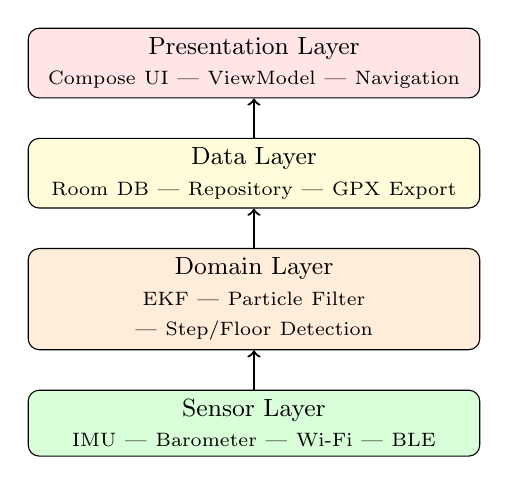
\begin{tikzpicture}[
    node distance=0.5cm,
    block/.style={rectangle, draw, fill=blue!10, text width=5.5cm, text centered, rounded corners, minimum height=0.8cm, font=\small},
    arrow/.style={->, thick}
]
    \node[block, fill=green!15] (sensor) {Sensor Layer\\{\scriptsize IMU | Barometer | Wi-Fi | BLE}};
    \node[block, fill=orange!15, above=of sensor] (domain) {Domain Layer\\{\scriptsize EKF | Particle Filter | Step/Floor Detection}};
    \node[block, fill=yellow!15, above=of domain] (data) {Data Layer\\{\scriptsize Room DB | Repository | GPX Export}};
    \node[block, fill=red!10, above=of data] (ui) {Presentation Layer\\{\scriptsize Compose UI | ViewModel | Navigation}};

    \draw[arrow] (sensor) -- (domain);
    \draw[arrow] (domain) -- (data);
    \draw[arrow] (data) -- (ui);
\end{tikzpicture}
\caption{Layered system architecture with unidirectional data flow.}
\label{fig:architecture}
\end{figure}

\subsection{Reactive Sensor Pipeline}

A key architectural innovation is the use of reactive data streams for sensor data processing. Each sensor collector implements a common interface that exposes a \texttt{Flow<SensorReading>}, enabling:
\begin{itemize}
    \item Automatic lifecycle management (collection starts/stops with subscribers)
    \item Back-pressure handling for high-rate sensors (50~Hz IMU)
    \item Composable transformation pipelines (filtering, mapping, combining)
    \item Thread-safe data sharing between sensor callbacks and processing algorithms
\end{itemize}

The sensor readings are modeled as a sealed class hierarchy with distinct subtypes for IMU, Pressure, Wi-Fi Scan, BLE Scan, and Step Event data, ensuring type safety throughout the processing pipeline.

\subsection{Dual-Filter Fusion Strategy}

The system employs a dual-filter architecture (Fig.~\ref{fig:fusion}) that leverages the complementary strengths of the Extended Kalman Filter and Particle Filter:

\begin{figure}[htbp]
\centering
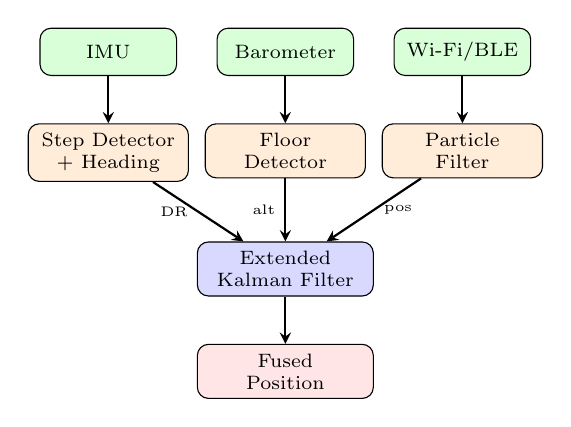
\begin{tikzpicture}[
    node distance=0.4cm and 0.3cm,
    sensor/.style={rectangle, draw, fill=green!15, text width=1.5cm, text centered, rounded corners, minimum height=0.6cm, font=\scriptsize},
    algo/.style={rectangle, draw, fill=orange!15, text width=1.8cm, text centered, rounded corners, minimum height=0.6cm, font=\scriptsize},
    filter/.style={rectangle, draw, fill=blue!15, text width=2cm, text centered, rounded corners, minimum height=0.6cm, font=\scriptsize},
    output/.style={rectangle, draw, fill=red!10, text width=2cm, text centered, rounded corners, minimum height=0.6cm, font=\scriptsize},
    arrow/.style={->, thick, >=stealth, font=\tiny}
]
    % Sensors
    \node[sensor] (imu) {IMU};
    \node[sensor, right=0.5cm of imu] (baro) {Barometer};
    \node[sensor, right=0.5cm of baro] (wifi) {Wi-Fi/BLE};

    % Algorithms
    \node[algo, below=0.6cm of imu] (step) {Step Detector\\+ Heading};
    \node[algo, below=0.6cm of baro] (floor) {Floor\\Detector};
    \node[algo, below=0.6cm of wifi] (pf) {Particle\\Filter};

    % EKF
    \node[filter, below=0.8cm of floor] (ekf) {Extended\\Kalman Filter};

    % Output
    \node[output, below=0.6cm of ekf] (pos) {Fused\\Position};

    % Arrows
    \draw[arrow] (imu) -- (step);
    \draw[arrow] (baro) -- (floor);
    \draw[arrow] (wifi) -- (pf);
    \draw[arrow] (step) -- (ekf) node[midway,left,font=\tiny] {DR};
    \draw[arrow] (floor) -- (ekf) node[midway,left,font=\tiny] {alt};
    \draw[arrow] (pf) -- (ekf) node[midway,right,font=\tiny] {pos};
    \draw[arrow] (ekf) -- (pos);
\end{tikzpicture}
\caption{Dual-filter sensor fusion architecture. The Particle Filter processes RF measurements and feeds position estimates to the EKF.}
\label{fig:fusion}
\end{figure}

\begin{itemize}
    \item The \textbf{EKF} maintains the primary state estimate, processing PDR measurements at high rate (50~Hz) and incorporating corrections from barometric altitude and RF-based positioning.
    \item The \textbf{Particle Filter} processes Wi-Fi and BLE measurements, naturally handling the multimodal and non-Gaussian distributions characteristic of RF propagation in complex indoor environments.
\end{itemize}

The Particle Filter estimate is fed into the EKF as a position measurement, weighted by the particle spread (uncertainty). This hierarchical approach avoids the computational complexity of running a single particle filter at IMU rates while preserving the PF's ability to handle ambiguous RF signals.

%===============================================================================
% IV. ALGORITHMS
%===============================================================================
\section{Positioning Algorithms}
\label{sec:algorithms}

\subsection{Extended Kalman Filter}

The EKF maintains an 8-dimensional state vector:
\begin{equation}
    \mathbf{x} = [x, y, z, v_x, v_y, v_z, \psi, f]^T
    \label{eq:state}
\end{equation}
where $(x, y, z)$ is the 3D position in a local Cartesian frame, $(v_x, v_y, v_z)$ are velocity components, $\psi$ is heading (azimuth), and $f$ is the current floor number.

\subsubsection{Prediction Step}
The state transition follows a constant-velocity model:
\begin{equation}
    \mathbf{x}_{k|k-1} = \mathbf{F}_k \mathbf{x}_{k-1|k-1}
    \label{eq:ekf_predict_state}
\end{equation}
\begin{equation}
    \mathbf{P}_{k|k-1} = \mathbf{F}_k \mathbf{P}_{k-1|k-1} \mathbf{F}_k^T + \alpha \mathbf{Q}
    \label{eq:ekf_predict_cov}
\end{equation}
where the state transition matrix is:
\begin{equation}
    \mathbf{F}_k = \mathbf{I}_8 + \Delta t \begin{bmatrix}
    \mathbf{0}_{3\times3} & \mathbf{I}_{3\times3} & \mathbf{0}_{3\times2} \\
    \mathbf{0}_{3\times3} & \mathbf{0}_{3\times3} & \mathbf{0}_{3\times2} \\
    \mathbf{0}_{2\times3} & \mathbf{0}_{2\times3} & \mathbf{0}_{2\times2}
    \end{bmatrix}
    \label{eq:transition}
\end{equation}

The parameter $\alpha$ is an adaptive process noise scaling factor:
\begin{equation}
    \alpha = \begin{cases}
    1.0 & \text{if step detected (walking)} \\
    0.1 & \text{if stationary}
    \end{cases}
    \label{eq:adaptive_noise}
\end{equation}

This adaptive scaling reduces position drift during stationary periods while allowing appropriate uncertainty growth during motion.

\subsubsection{Update Step}
The update step employs the Joseph form for numerical stability:
\begin{equation}
    \mathbf{y}_k = \mathbf{z}_k - \mathbf{H}_k \mathbf{x}_{k|k-1}
    \label{eq:innovation}
\end{equation}
\begin{equation}
    \mathbf{S}_k = \mathbf{H}_k \mathbf{P}_{k|k-1} \mathbf{H}_k^T + \mathbf{R}_k
    \label{eq:innovation_cov}
\end{equation}
\begin{equation}
    \mathbf{K}_k = \mathbf{P}_{k|k-1} \mathbf{H}_k^T \mathbf{S}_k^{-1}
    \label{eq:kalman_gain}
\end{equation}
\begin{equation}
    \mathbf{x}_{k|k} = \mathbf{x}_{k|k-1} + \mathbf{K}_k \mathbf{y}_k
    \label{eq:state_update}
\end{equation}
\begin{equation}
    \mathbf{P}_{k|k} = (\mathbf{I} - \mathbf{K}_k \mathbf{H}_k) \mathbf{P}_{k|k-1} (\mathbf{I} - \mathbf{K}_k \mathbf{H}_k)^T + \mathbf{K}_k \mathbf{R}_k \mathbf{K}_k^T
    \label{eq:joseph}
\end{equation}

The Joseph form (\ref{eq:joseph}) is preferred over the standard formulation $\mathbf{P} = (\mathbf{I} - \mathbf{KH})\mathbf{P}$ because it guarantees positive semi-definiteness of the covariance matrix even under finite-precision arithmetic \cite{bucy1968digital}.

The EKF accepts multiple measurement types with different observation matrices $\mathbf{H}$ and noise covariances $\mathbf{R}$:

\begin{itemize}
    \item \textbf{Dead Reckoning}: $\mathbf{H}_{DR} \in \mathbb{R}^{2 \times 8}$ observing $(x, y)$, with $\mathbf{R}_{DR} = 0.5\mathbf{I}_2$ m$^2$.
    \item \textbf{Barometric Altitude}: $\mathbf{H}_{alt} \in \mathbb{R}^{1 \times 8}$ observing $z$, with $R_{alt} = 2.0$ m$^2$.
    \item \textbf{GPS}: $\mathbf{H}_{GPS} \in \mathbb{R}^{3 \times 8}$ observing $(x, y, z)$, with $R_{GPS} = \sigma_{acc}^2$ based on reported accuracy.
    \item \textbf{Particle Filter}: $\mathbf{H}_{PF} \in \mathbb{R}^{2 \times 8}$ observing $(x, y)$, with $R_{PF} = \sigma_{spread}^2$ proportional to particle cloud spread.
\end{itemize}

\subsection{Particle Filter}

The Particle Filter represents the posterior position distribution as a set of $N$ weighted samples (particles):
\begin{equation}
    \{(\mathbf{x}_k^{(i)}, w_k^{(i)})\}_{i=1}^{N}, \quad \sum_{i=1}^N w_k^{(i)} = 1
    \label{eq:particles}
\end{equation}

Each particle $\mathbf{x}^{(i)} = [x^{(i)}, y^{(i)}, z^{(i)}, \psi^{(i)}, f^{(i)}]$ represents a position hypothesis with associated weight.

\subsubsection{Motion Model}
Particles are propagated using a stochastic dead reckoning model:
\begin{equation}
    x_k^{(i)} = x_{k-1}^{(i)} + (L + \epsilon_L) \cos(\psi + \epsilon_\psi)
    \label{eq:pf_motion_x}
\end{equation}
\begin{equation}
    y_k^{(i)} = y_{k-1}^{(i)} + (L + \epsilon_L) \sin(\psi + \epsilon_\psi)
    \label{eq:pf_motion_y}
\end{equation}
where $L$ is the estimated stride length, $\psi$ is the estimated heading, and $\epsilon_L \sim \mathcal{N}(0, \sigma_L^2)$, $\epsilon_\psi \sim \mathcal{N}(0, \sigma_\psi^2)$ are process noise terms.

\subsubsection{Wi-Fi RSSI Measurement Model}
Particle weights are updated based on the log-distance path loss model. The likelihood of observing RSSI value $r_j$ from access point $j$ given particle position $\mathbf{x}^{(i)}$ is:
\begin{equation}
    p(r_j | \mathbf{x}^{(i)}) = \frac{1}{\sqrt{2\pi}\sigma_r} \exp\left(-\frac{(r_j - \hat{r}_j^{(i)})^2}{2\sigma_r^2}\right)
    \label{eq:rssi_likelihood}
\end{equation}
where the expected RSSI is:
\begin{equation}
    \hat{r}_j^{(i)} = A - 10n\log_{10}\left(\|\mathbf{x}^{(i)} - \mathbf{p}_j\|\right)
    \label{eq:expected_rssi}
\end{equation}
and $\sigma_r \approx 5$~dBm captures the RSSI measurement noise.

The combined weight update for $M$ observed access points is:
\begin{equation}
    w_k^{(i)} \propto w_{k-1}^{(i)} \prod_{j=1}^{M} p(r_j | \mathbf{x}^{(i)})
    \label{eq:weight_update}
\end{equation}

\subsubsection{Wi-Fi RTT Measurement Model}
For access points supporting IEEE 802.11mc, the measured distance $d_j$ provides a more direct observation:
\begin{equation}
    p(d_j | \mathbf{x}^{(i)}) = \frac{1}{\sqrt{2\pi}\sigma_d} \exp\left(-\frac{(d_j - \|\mathbf{x}^{(i)} - \mathbf{p}_j\|)^2}{2\sigma_d^2}\right)
    \label{eq:rtt_likelihood}
\end{equation}
where $\sigma_d \approx 1.0$--$1.5$~m is the RTT ranging noise standard deviation.

\subsubsection{Systematic Resampling}
When the effective sample size $N_{eff}$ drops below a threshold:
\begin{equation}
    N_{eff} = \frac{1}{\sum_{i=1}^N (w_k^{(i)})^2} < \gamma N
    \label{eq:neff}
\end{equation}
with $\gamma = 0.5$, systematic resampling is performed. This method generates $N$ new particles by stratified sampling from the cumulative weight distribution, providing lower variance than multinomial resampling \cite{gustafsson2010particle}.

\subsection{Adaptive Step Detection}

The step detection algorithm operates on the acceleration magnitude signal:
\begin{equation}
    a_m[k] = \sqrt{a_x[k]^2 + a_y[k]^2 + a_z[k]^2}
    \label{eq:accel_mag}
\end{equation}

A low-pass filter smooths the signal:
\begin{equation}
    \tilde{a}_m[k] = \alpha_f \cdot a_m[k] + (1 - \alpha_f) \cdot \tilde{a}_m[k-1]
    \label{eq:lowpass}
\end{equation}
with $\alpha_f = 0.2$.

\subsubsection{Dynamic Threshold}
Unlike fixed-threshold approaches, the system computes an adaptive threshold from the recent signal statistics:
\begin{equation}
    \tau[k] = \bar{a}_m + 0.8 \cdot \sigma_{a_m}
    \label{eq:threshold}
\end{equation}
where $\bar{a}_m$ and $\sigma_{a_m}$ are the mean and standard deviation of the acceleration magnitude over a sliding window of 50 samples.

\subsubsection{Peak-Valley Detection}
Steps are detected through a state machine that identifies alternating peaks and valleys:
\begin{enumerate}
    \item \textbf{Peak search}: Track the maximum value until a decline of $>0.5$~m/s$^2$ is observed with peak above $\tau[k]$.
    \item \textbf{Valley search}: Track the minimum value until a rise of $>0.5$~m/s$^2$ is observed.
    \item \textbf{Step validation}: Ensure the inter-step interval is within $[250, 2000]$~ms.
\end{enumerate}

\subsubsection{Weinberg Stride Length}
The stride length is estimated using the Weinberg model (\ref{eq:weinberg}) with calibration constant $K = 0.52$ and output clamped to $[0.3, 1.5]$~m to prevent unreasonable estimates.

\subsection{Heading Estimation}

Heading is estimated using a complementary filter that fuses gyroscope integration (short-term accuracy) with tilt-compensated magnetometer heading (long-term stability):
\begin{equation}
    \psi[k] = \alpha_c \cdot (\psi[k-1] + \omega_z \cdot \Delta t) + (1 - \alpha_c) \cdot \psi_{mag}[k]
    \label{eq:complementary}
\end{equation}
where $\alpha_c = 0.98$ weights the gyroscope heavily for smooth short-term tracking, while the magnetometer prevents long-term drift.

The tilt-compensated magnetic heading $\psi_{mag}$ is computed from the rotation matrix obtained via the accelerometer and magnetometer readings, following the standard Android sensor fusion API.

\subsection{Barometric Floor Detection}

Floor detection uses the hypsometric formula (\ref{eq:hypsometric}) to convert pressure to altitude, followed by moving-average smoothing:
\begin{equation}
    \bar{h}[k] = \frac{1}{W} \sum_{i=k-W+1}^{k} h[i]
    \label{eq:moving_avg}
\end{equation}
with window size $W = 30$ samples.

Floor transitions are detected when the smoothed altitude change from the last detected floor exceeds a threshold:
\begin{equation}
    \Delta f = \text{round}\left(\frac{\bar{h}[k] - h_{ref}}{h_{floor}}\right)
    \label{eq:floor_change}
\end{equation}
where $h_{floor} = 3.0$~m is the nominal floor height and $h_{ref}$ is the altitude at the last floor change.

The transition threshold is activity-dependent:
\begin{equation}
    \tau_h = \begin{cases}
    2.0 \text{ m} & \text{general motion} \\
    1.6 \text{ m} & \text{stair climbing detected} \\
    1.2 \text{ m} & \text{elevator detected}
    \end{cases}
    \label{eq:floor_threshold}
\end{equation}

Floor detection confidence is computed from pressure stability:
\begin{equation}
    c = 1 - \min\left(\frac{\sigma_P^2}{1.0}, 1.0\right)
    \label{eq:confidence}
\end{equation}
where $\sigma_P^2$ is the variance of recent pressure readings.

%===============================================================================
% V. IMPLEMENTATION
%===============================================================================
\section{Implementation}
\label{sec:implementation}

\subsection{Technology Stack}

The system is implemented as an Android application targeting API level 26+ (Android 8.0 Oreo) with the technology stack summarized in Table~\ref{tab:techstack}.

\begin{table}[htbp]
\caption{Technology Stack}
\label{tab:techstack}
\centering
\begin{tabular}{@{}ll@{}}
\toprule
\textbf{Component} & \textbf{Technology} \\
\midrule
Language & Kotlin 1.9 \\
Build System & Gradle KTS \\
Async/Reactive & Coroutines + Flow \\
UI Framework & Jetpack Compose (Material 3) \\
DI Framework & Hilt (Dagger) \\
Database & Room \\
Math Library & Apache Commons Math 3.6 \\
Location & Google FusedLocationProvider \\
BLE & Nordic Semiconductor BLE Library \\
Architecture & MVVM + Clean Architecture \\
\bottomrule
\end{tabular}
\end{table}

\subsection{Sensor Data Pipeline}

Each hardware sensor is abstracted behind a \texttt{SensorCollector<T>} interface that produces a Kotlin Flow of typed sensor readings. The reactive pipeline architecture ensures:

\begin{itemize}
    \item \textbf{Lifecycle awareness}: Sensor registration and unregistration are tied to Flow collection, preventing resource leaks.
    \item \textbf{Backpressure}: The \texttt{callbackFlow} builder with \texttt{trySend} handles the case where the consumer cannot keep up with the producer.
    \item \textbf{Thread safety}: Flow operators handle context switching between sensor callback threads and processing coroutines.
\end{itemize}

The IMU collector fuses accelerometer, gyroscope, and magnetometer data into a single \texttt{Imu} reading emitted at accelerometer rate (~50~Hz). Barometer readings are emitted at UI rate (~5~Hz). Wi-Fi scans are triggered at ~1~Hz, and BLE scans are batched at 1-second intervals.

\subsection{Coordinate System}

Position calculations are performed in a local East-North-Up (ENU) Cartesian coordinate system centered at a reference point. The conversion between geographic (latitude/longitude) and local coordinates uses a Mercator approximation valid for small areas:
\begin{equation}
    x = (lon - lon_0) \cdot \frac{\pi}{180} \cdot R_E \cdot \cos(lat)
    \label{eq:lon_to_m}
\end{equation}
\begin{equation}
    y = (lat - lat_0) \cdot \frac{\pi}{180} \cdot R_E
    \label{eq:lat_to_m}
\end{equation}
where $R_E = 6{,}371{,}000$~m is the Earth's mean radius and $(lat_0, lon_0)$ is the reference point.

\subsection{Data Persistence}

Position records are stored in a Room database with a streamlined schema containing 20 fields per record (compared to 46+ in the legacy system). The schema captures position, motion state, sensor readings, floor information, and session metadata. Records are grouped by session identifiers enabling track replay and GPX export.

\subsection{Foreground Service}

Continuous positioning in the background is achieved through an Android foreground service with location type, ensuring sensor data collection continues when the application UI is not visible. The service manages the lifecycle of all sensor collectors and the positioning engine.

%===============================================================================
% VI. COMPARATIVE ANALYSIS
%===============================================================================
\section{Comparative Analysis with Legacy System}
\label{sec:comparison}

The proposed system represents a comprehensive redesign of an earlier indoor positioning application. Table~\ref{tab:comparison} summarizes the key differences.

\begin{table}[htbp]
\caption{Legacy vs. Modern System Comparison}
\label{tab:comparison}
\centering
\small
\begin{tabular}{@{}p{2.2cm}p{2.5cm}p{2.5cm}@{}}
\toprule
\textbf{Aspect} & \textbf{Legacy} & \textbf{Modern} \\
\midrule
Language & Java & Kotlin \\
Min SDK & API 15 & API 26 \\
Build & Maven & Gradle KTS \\
UI & XML + ActionBar Sherlock & Jetpack Compose (M3) \\
DI & Manual & Hilt \\
Database & Raw SQLite (46+ cols) & Room (20 cols) \\
Async & Thread + Timer & Coroutines + Flow \\
Matrix Library & EJML (10K+ LOC source) & Commons Math (dep) \\
\midrule
\multicolumn{3}{@{}l}{\textit{Positioning Algorithms}} \\
\midrule
Kalman Filter & 3 separate basic KF & Single EKF (Joseph) \\
RF Positioning & None & Particle Filter \\
Step Detection & Basic peak counting & Adaptive threshold + Weinberg \\
Floor Detection & Linear $\Delta P/12$ & Hypsometric formula \\
Wi-Fi & Not used & RSSI + RTT (802.11mc) \\
BLE & TI SensorTag only & Universal iBeacon/ Eddystone \\
Heading & None & Complementary filter \\
\midrule
Source Files & 205 (incl. EJML) & 38 \\
\bottomrule
\end{tabular}
\end{table}

\subsection{Algorithmic Improvements}

\subsubsection{Kalman Filter}
The legacy system contained three separate Kalman filter implementations (\texttt{KalmanFilterSimple}, \texttt{KalmanFilterOperations}, \texttt{KalmanFilterEquation}) using the EJML matrix library included as full source code (90+ classes, 10,000+ lines). The modern system replaces all three with a single Extended Kalman Filter implementation that:
\begin{itemize}
    \item Supports non-linear measurement models via Jacobian linearization
    \item Uses the Joseph form for guaranteed positive semi-definite covariance
    \item Employs adaptive process noise based on motion state
    \item Uses Apache Commons Math as a maintained external dependency
\end{itemize}

\subsubsection{RF-Based Positioning}
The legacy system relied exclusively on GPS and cell tower positioning with no Wi-Fi or BLE-based indoor positioning capability. The modern system introduces a Particle Filter that processes both RSSI-based proximity estimates and Wi-Fi RTT distance measurements, enabling meter-level indoor positioning.

\subsubsection{Step Detection}
The legacy system used basic accelerometer peak detection without adaptive thresholding or stride length estimation. The modern system implements:
\begin{itemize}
    \item Dynamic threshold adaptation based on signal statistics
    \item Weinberg model for stride length estimation
    \item State-machine-based peak-valley detection with minimum step period enforcement
    \item Step frequency estimation for activity classification
\end{itemize}

\subsubsection{Floor Detection}
The legacy system used a linear approximation of 12~Pa per meter of altitude change, which introduces approximately 2\% error at sea level and increasing error at higher elevations. The modern system uses the full hypsometric formula (\ref{eq:hypsometric}), providing altitude accuracy within 0.1~m across the range of typical building heights.

\subsection{Architectural Improvements}

\subsubsection{Modularity}
The legacy system exhibited tight coupling between UI components, sensor management, and positioning logic within a monolithic service class (\texttt{GpsLoggingService.java}, ~800 lines). The modern system separates concerns across distinct layers with well-defined interfaces, enabling independent testing and modification of each component.

\subsubsection{Testability}
The legacy system contained no unit tests. The modern system includes comprehensive unit tests for all core algorithms:
\begin{itemize}
    \item EKF: state initialization, prediction, update convergence, uncertainty reduction
    \item Particle Filter: initialization, motion propagation, RSSI/RTT updates, floor constraints
    \item Step Detector: stationary rejection, walking detection, stride range validation
    \item Floor Detector: stability, transition detection, reference calibration, confidence
\end{itemize}

\subsubsection{Code Reduction}
The legacy system comprised 205 Java source files (including the full EJML library). The modern system achieves equivalent and extended functionality in 38 Kotlin files (3,451 lines), representing a 5.4$\times$ reduction in file count while adding Particle Filter, Wi-Fi RTT, and BLE positioning capabilities.

\subsection{Expected Performance Characteristics}

Based on the algorithmic foundations and measurement models employed, the system's expected positioning performance characteristics are summarized in Table~\ref{tab:performance}.

\begin{table}[htbp]
\caption{Expected Positioning Performance}
\label{tab:performance}
\centering
\begin{tabular}{@{}lcc@{}}
\toprule
\textbf{Configuration} & \textbf{Horizontal} & \textbf{Vertical} \\
\midrule
PDR only & 5--10 m (drift) & N/A \\
PDR + Barometer & 5--10 m & Floor-level \\
PDR + Wi-Fi RSSI & 3--5 m & Floor-level \\
PDR + Wi-Fi RTT & 1--2 m & Floor-level \\
PDR + BLE + Wi-Fi RTT & $<$2 m & Floor-level \\
Full fusion (all sensors) & 1--3 m & $>$90\% floor \\
\bottomrule
\end{tabular}
\end{table}

%===============================================================================
% VII. CONCLUSION
%===============================================================================
\section{Conclusion}
\label{sec:conclusion}

This paper presented a modern multi-sensor fusion architecture for indoor positioning that integrates pedestrian dead reckoning, barometric floor detection, Wi-Fi RTT ranging, and BLE beacon proximity within a dual Extended Kalman Filter and Particle Filter framework. The system represents a complete redesign of a legacy indoor positioning application, leveraging modern mobile development paradigms and improved positioning algorithms.

The key contributions of this work are:
\begin{enumerate}
    \item A \textbf{dual-filter fusion architecture} that combines the computational efficiency of the EKF for high-rate IMU processing with the distributional flexibility of the Particle Filter for RF-based measurements.
    \item An \textbf{adaptive step detection algorithm} using the Weinberg stride length model and dynamic thresholding, providing improved dead reckoning accuracy across different walking speeds and gaits.
    \item A \textbf{hypsometric formula-based floor detector} with activity-dependent transition thresholds, improving vertical positioning accuracy over linear approximations.
    \item A \textbf{clean layered architecture} with reactive sensor pipelines that reduces code complexity by 5.4$\times$ while extending positioning capabilities with Wi-Fi RTT and BLE support.
\end{enumerate}

Future work will focus on: (1) integration of map constraints into the Particle Filter to prevent impossible positions (through walls), (2) machine learning-based activity recognition using CNN or LSTM networks applied to raw IMU data, (3) collaborative positioning using crowd-sourced sensor data, and (4) support for Ultra-Wideband (UWB) ranging when hardware becomes widely available.

%===============================================================================
% REFERENCES
%===============================================================================
\begin{thebibliography}{20}

\bibitem{zafari2019survey}
F. Zafari, A. Gkelias, and K. K. Leung, ``A survey of indoor localization systems and technologies,'' \textit{IEEE Communications Surveys \& Tutorials}, vol. 21, no. 3, pp. 2568--2599, 2019.

\bibitem{groves2013principles}
P. D. Groves, \textit{Principles of GNSS, Inertial, and Multisensor Integrated Navigation Systems}, 2nd ed. Boston, MA: Artech House, 2013.

\bibitem{davidson2017survey}
P. Davidson and R. Pich\'{e}, ``A survey of selected indoor positioning methods for smartphones,'' \textit{IEEE Communications Surveys \& Tutorials}, vol. 19, no. 2, pp. 1347--1370, 2017.

\bibitem{he2016wifi}
S. He and S.-H. G. Chan, ``Wi-Fi fingerprint-based indoor positioning: Recent advances and comparisons,'' \textit{IEEE Communications Surveys \& Tutorials}, vol. 18, no. 1, pp. 466--490, 2016.

\bibitem{harle2013survey}
R. Harle, ``A survey of indoor inertial positioning systems for pedestrians,'' \textit{IEEE Communications Surveys \& Tutorials}, vol. 15, no. 3, pp. 1281--1293, 2013.

\bibitem{weinberg2002using}
H. Weinberg, ``Using the ADXL202 in pedometer and personal navigation applications,'' \textit{Analog Devices, Application Note AN-602}, 2002.

\bibitem{tian2015enhanced}
Q. Tian, Z. Salcic, K. I.-K. Wang, and Y. Pan, ``An enhanced pedestrian dead reckoning approach for pedestrian tracking using smartphones,'' in \textit{Proc. IEEE 10th Conf. Ind. Electron. Appl. (ICIEA)}, 2015, pp. 488--493.

\bibitem{muralidharan2014barometric}
K. Muralidharan, A. J. Khan, A. Misra, R. K. Balan, and S. Nandi, ``Barometric phone sensors: More hype than hope!,'' in \textit{Proc. 15th Workshop Mobile Comput. Syst. Appl. (HotMobile)}, 2014, pp. 1--6.

\bibitem{xia2015altitude}
H. Xia, X. Wang, Y. Qiao, J. Jian, and Y. Chang, ``Using multiple barometers to detect the floor location of smart phones with built-in barometric sensors for indoor positioning,'' \textit{Sensors}, vol. 15, no. 4, pp. 7857--7877, 2015.

\bibitem{ibrahim2018verification}
M. Ibrahim, H. Liu, M. Jawahar, V. Nguyen, M. Gruteser, R. Howard, B. Yu, and F. Bai, ``Verification: Accuracy evaluation of WiFi fine time measurements on an open platform,'' in \textit{Proc. 24th Annu. Int. Conf. Mobile Comput. Netw. (MobiCom)}, 2018, pp. 417--427.

\bibitem{gustafsson2010particle}
F. Gustafsson, ``Particle filter theory and practice with positioning applications,'' \textit{IEEE Aerospace and Electronic Systems Magazine}, vol. 25, no. 7, pp. 53--82, 2010.

\bibitem{chen2015fusion}
Z. Chen, H. Zou, H. Jiang, Q. Zhu, Y. C. Soh, and L. Xie, ``Fusion of WiFi, smartphone sensors and landmarks using the Kalman filter for indoor localization,'' \textit{Sensors}, vol. 15, no. 1, pp. 715--732, 2015.

\bibitem{bucy1968digital}
R. S. Bucy and P. D. Joseph, \textit{Filtering for Stochastic Processes with Applications to Guidance}. New York: Interscience Publishers, 1968.

\bibitem{dalgin_legacy}
S. Dalgin, ``LBS/DR: Location based services with dead reckoning for indoor positioning,'' Unpublished software, Istanbul, Turkey, 2014.

\end{thebibliography}

\end{document}
